\documentclass[11pt]{article}
\usepackage[margin=1in]{geometry}
\usepackage[T1]{fontenc}
\usepackage{lmodern}
\usepackage{amsmath,amssymb,booktabs,array,graphicx}
\usepackage{hyperref}
\hypersetup{colorlinks=true,linkcolor=blue,urlcolor=blue,citecolor=blue,
  pdftitle={A replication of Chumney (2013) on small-sample SEM estimators},
  pdfauthor={}}
\renewcommand{\arraystretch}{1.35}
\newcommand{\codebase}{https://github.com/alectionary/vibe-math/blob/master/formalization/chumney-sem-small-samples}
\newcommand{\code}[2]{\href{\codebase/#1\#L#2}{\texttt{#1:#2}}}
\newcommand{\filelink}[1]{\href{\codebase/#1}{\texttt{#1}}}
\begingroup
\catcode`\_=12
\gdef\linkcsv{\href{https://github.com/alectionary/vibe-math/blob/master/formalization/chumney-sem-small-samples/simulation/out/comparison_i3.csv}{\texttt{simulation/out/comparison_i3.csv}}}
\gdef\linkcheck{\href{https://github.com/alectionary/vibe-math/blob/master/formalization/chumney-sem-small-samples/simulation/check_standardized.R}{\texttt{simulation/check_standardized.R}}}
\gdef\linkcrop{\href{https://github.com/alectionary/vibe-math/blob/master/formalization/chumney-sem-small-samples/paper/figures/crop_pages.py}{\texttt{paper/figures/crop_pages.py}}}
\gdef\linkbayes{\href{https://github.com/alectionary/vibe-math/blob/master/formalization/chumney-sem-small-samples/simulation/bayes_subset.R}{\texttt{simulation/bayes_subset.R}}}
\gdef\linkform{\href{https://github.com/alectionary/vibe-math/blob/master/formalization/chumney-sem-small-samples/simulation/investigate_formative.R}{\texttt{investigate\_formative.R}}}
\gdef\linkformout{\href{https://github.com/alectionary/vibe-math/blob/master/formalization/chumney-sem-small-samples/simulation/out/formative_readings.txt}{\texttt{formative\_readings.txt}}}
\gdef\linkgsca{\href{https://github.com/alectionary/vibe-math/blob/master/formalization/chumney-sem-small-samples/simulation/investigate_gsca.R}{\texttt{investigate\_gsca.R}}}
\gdef\linkgscaout{\href{https://github.com/alectionary/vibe-math/blob/master/formalization/chumney-sem-small-samples/simulation/out/gsca_compare.rds}{\texttt{gsca\_compare.rds}}}
\endgroup

\title{A replication of Chumney (2013):\\
four estimators for structural equation models with small samples}
\author{}
\date{29 October 2026}

\begin{document}
\maketitle

\begin{abstract}
Which estimator recovers a three-factor structural equation model when the
sample is small? Chumney (2013) compared maximum likelihood, partial least
squares, generalized structured component analysis, and Bayesian Markov chain
Monte Carlo on normal data, and concluded that maximum likelihood is generally
the most robust of the four and the approach of choice for applied
researchers. We regenerated the 36 data conditions and refit maximum likelihood, partial
least squares, and generalized structured component analysis, with 150
replications in each cell. A documented Bayesian subset, 30 replications
at the sample sizes 50 and 1000, was fit in blavaan with a 1000-iteration
cap. Maximum likelihood and the Bayesian estimator have similar percent
bias, and both are more accurate than the two component methods on
reflective measurement parameters. The printed seven-indicator rise in
generalized structured component analysis is absent from both R
implementations we ran. One printed maximum likelihood cell, structural
percent bias 1.196, was not reproduced under the readings we tried.
\end{abstract}

\section{The headline}
\label{sec:headline}

Does maximum likelihood dominate the other three estimators on normal data
from this three-factor model? The comparison is a partial match. On
reflective measurement percent bias, maximum likelihood and the Bayesian
estimator sit together near 2.7 to 2.9 at $n=1000$, and partial least
squares and generalized structured component analysis sit near 15.9. The
dissertation's own exceptions, where the component methods are less biased
for the paths, are reproduced. The runs do not separate maximum likelihood
from the Bayesian estimator.

Chumney's dissertation asks how sample size, the number of items, omitted
cross-loadings, and reflective versus formative indicators change the
behavior of four estimators. The closing paragraph of Chapter~5 states the
result that the abstract also states. Figure~\ref{fig:headline} is that
paragraph. The sentence is: maximum likelihood is generally the most robust
of the four, and it should be the approach of choice, with the dependence on
the normal data and the models in the study kept in view.

\begin{figure}[ht]
\centering
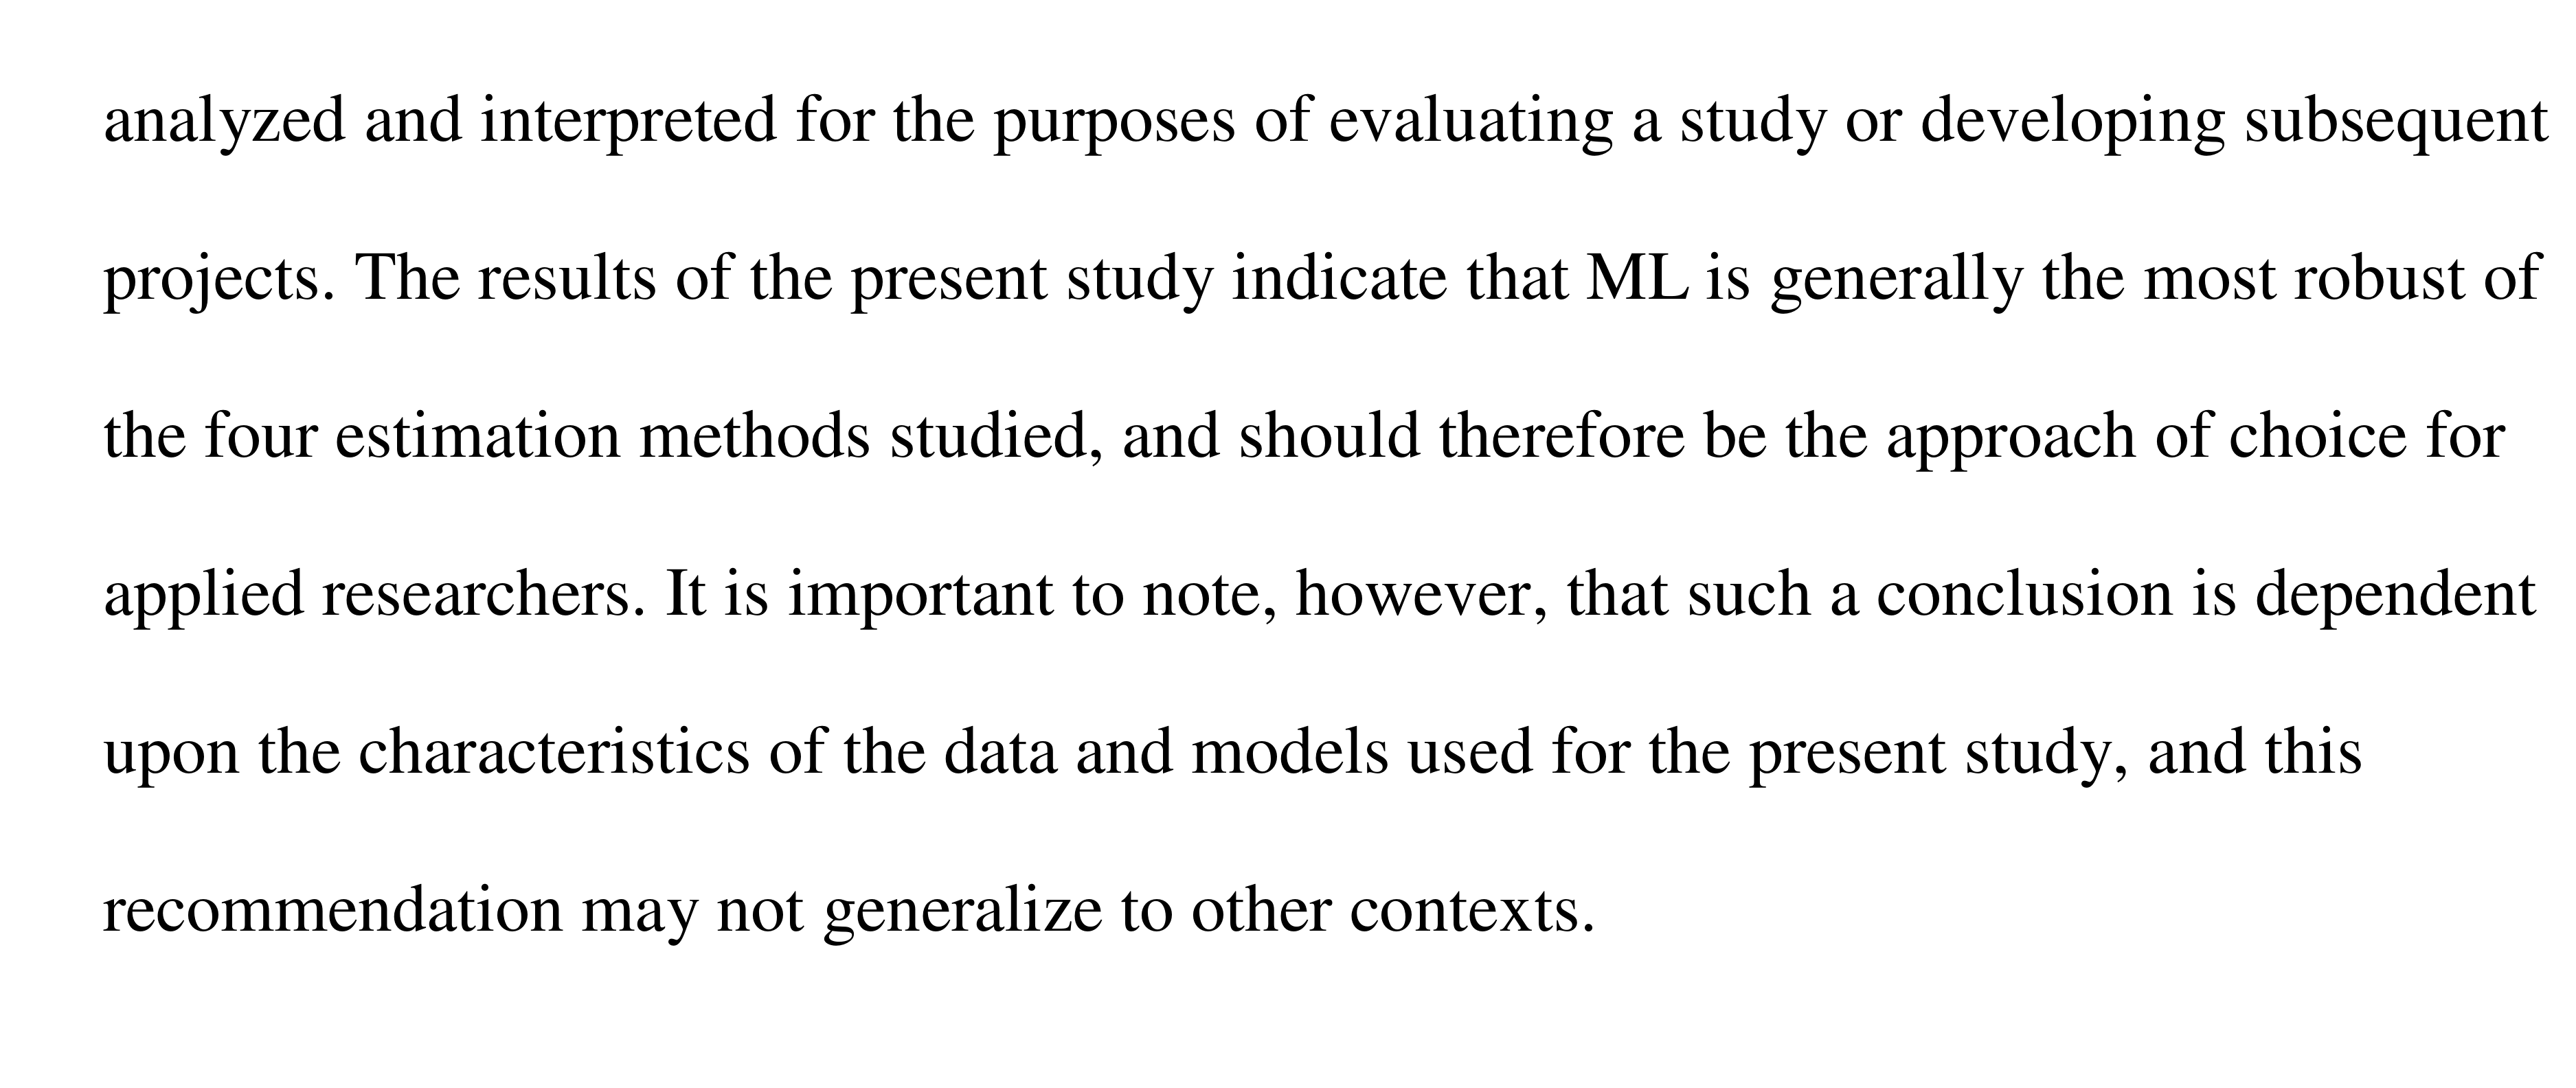
\includegraphics[width=\textwidth]{figures/headline.png}
\caption{Chumney (2013), dissertation page 118. The headline sentence is
the one that names maximum likelihood as generally the most robust of the
four methods.}
\label{fig:headline}
\end{figure}

Table~\ref{tab:compare} is the comparison. A match means the difference of
Monte Carlo means lies inside a two-standard-error band and is not rejected
by a Holm adjustment within that outcome on the three-indicator slice.
Percent bias is equation~(15), the absolute relative error times 100,
averaged over the loadings or over the two paths. The goodness-of-fit row
uses the benchmark $\sqrt{1 \times 0.36} = 0.600$, discussed in
Section~\ref{sec:gof}. Counts of converged replications are out of 150.

\begin{table}[ht]
\centering
\caption{Printed claims and our Monte Carlo means. The three-indicator
cells are from Tables~1--4. The seven-indicator cells are from Tables~3
and~4. Standard errors and the Holm labels are in
\linkcsv.}
\label{tab:compare}
\small
\begin{tabular}{@{}p{0.30\textwidth}p{0.20\textwidth}p{0.22\textwidth}p{0.16\textwidth}@{}}
\toprule
Claim & Published & Ours & Verdict \\
\midrule
ML measurement bias, $n=1000$, correct, reflective & 2.712 & 2.730 & Match \\
PLS measurement bias, same cell & 15.896 & 15.919 & Match \\
GSCA measurement bias, same cell & 15.918 & 15.938 & Match \\
ML structural bias, same cell & 4.203 & 4.106 & Match \\
PLS structural bias, misspecified reflective, $n=1000$ & 7.823 & 7.884 & Match \\
ML structural bias, same misspecified cell & 15.652 & 15.203 & Match \\
ML measurement bias, misspecified reflective, $n=1000$ & 9.673 & 9.676 & Match \\
ML measurement bias, misspecified formative, $n=1000$ & 21.643 & 21.686 & Match \\
PLS and GSCA convergence, all 36 conditions & 5400/5400 & 5400/5400 & Match \\
ML GoF bias, correct reflective, $n=1000$, minus 0.600 & $-0.180$ & $-0.179$ & Match \\
ML GoF bias, same cell, minus the standardized population value 0.420 & $-0.180$ & $+0.001$ & No match \\
ML convergence, misspecified formative, $n=50$ & 35 & 21 & Close \\
ML convergence, misspecified formative, $n=1000$ & 119 & 102 & Close \\
ML structural bias, correct formative, $n=1000$, three items & 1.196 & 2.601 & No match \\
ML structural bias, same row, five items & 2.623 & 2.516 & Match \\
ML structural bias, same row, seven items & 2.623 & 2.628 & Match \\
GSCA measurement bias, correct reflective, $n=1000$, seven items & 13.667 & 7.189 & No match \\
cSEM GSCA, same seven-item cell, 40 replications & 13.667 & 7.040 & No match \\
ML convergence, misspecified reflective, $n=50$, seven items & 102 & 150 & No match \\
\bottomrule
\end{tabular}
\end{table}

Table~\ref{tab:bayes} is the Bayesian subset. Thirty replications, two
chains, 500 burn-in iterations and 500 retained draws, potential scale
reduction below 1.05. The printed counts are out of 150. Ours are out of
30, so the convergence comparison is on the proportion.

\begin{table}[ht]
\centering
\caption{Bayesian subset against the printed Markov chain Monte Carlo
column. Measurement percent bias uses equation~(15).}
\label{tab:bayes}
\small
\begin{tabular}{@{}p{0.32\textwidth}p{0.18\textwidth}p{0.22\textwidth}p{0.16\textwidth}@{}}
\toprule
Claim & Published & Ours & Verdict \\
\midrule
MCMC measurement bias, $n=1000$, three items, correct, reflective & 2.738 & 2.902 & Match \\
MCMC structural bias, same cell & 4.272 & 3.847 & Match \\
MCMC measurement bias, $n=50$, seven items, correct, reflective & 10.202 & 10.596 & Match \\
MCMC convergence, same seven-item cell & 51/150 & 30/30 & No match \\
MCMC convergence, $n=50$, three items, misspecified formative & 149/150 & 22/30 & No match \\
Bayes measurement bias vs printed ML, $n=1000$, misspecified formative & 21.643 & 21.481 & Close \\
\bottomrule
\end{tabular}
\end{table}

The first measurement row is the headline comparison in numbers. At
$n=1000$ with three reflective indicators and a correct model, maximum
likelihood's mean absolute percent bias is 2.730, the Bayesian subset is
2.902, and the two component methods are 15.919 and 15.938. The printed
maximum likelihood and Markov chain Monte Carlo values in that cell are
2.712 and 2.738. Section~\ref{sec:bayes} gives the iteration cap and the
prior. Section~\ref{sec:matched} records the same ordering at five and
seven indicators for maximum likelihood and partial least squares.

The misspecified reflective structural rows are the exception Chapter~5
states in words: partial least squares and generalized structured component
analysis are less biased than maximum likelihood for the paths when
cross-loadings are omitted. Our means keep that order, 7.884 and 7.917
against 15.203, next to the printed 7.823, 7.791, and 15.652.

The goodness-of-fit pair is one printed number, $-0.180$, under two
benchmarks. Subtracting 0.600 from our mean goodness of fit reproduces
$-0.179$. Subtracting the standardized population value 0.420 produces
$+0.001$. Section~\ref{sec:gof} says what 0.600 is.

The formative structural row at three items and $n=1000$ stays at 2.601
under every reading in Section~\ref{sec:formative}. The five-item and
seven-item cells of that same printed row are 2.623 and 2.623, and our
means are 2.516 and 2.628.

The seven-indicator generalized structured component analysis rows are
where the printed column and the R implementations separate.
Section~\ref{sec:gsca7} records that gesca and cSEM's GSCA agree with each
other, at 7.189 and 7.040, while the printed value rises to 13.667.

\section{What we did ourselves, and what we took from others}
\label{sec:did}

This section answers what is ours and what is Chumney's. The model, the
$3 \times 3 \times 2 \times 2 \times 4$ design, and Tables~1--9 are the
dissertation's. The population covariance, the 150-replication Monte Carlo,
and Table~\ref{tab:compare} are ours.

The population model is a chain of three factors. The paths are 0.60. In the
marker scaling used to draw the data, each factor variance is 0.49, each
structural disturbance variance is 0.3136, and a simple reflective loading
is 1 with unique variance 0.51. Those numbers are the unstandardized
parameters whose standardized values are the ones named in the text: loadings
0.70, unique variances 0.51, disturbances 0.64. Figure~\ref{fig:population}
is the paragraph that states the standardized values. The figure above that
paragraph prints the marker scaling, including a disturbance of 0.31, which
is 0.3136 rounded to two decimals.

\begin{figure}[ht]
\centering
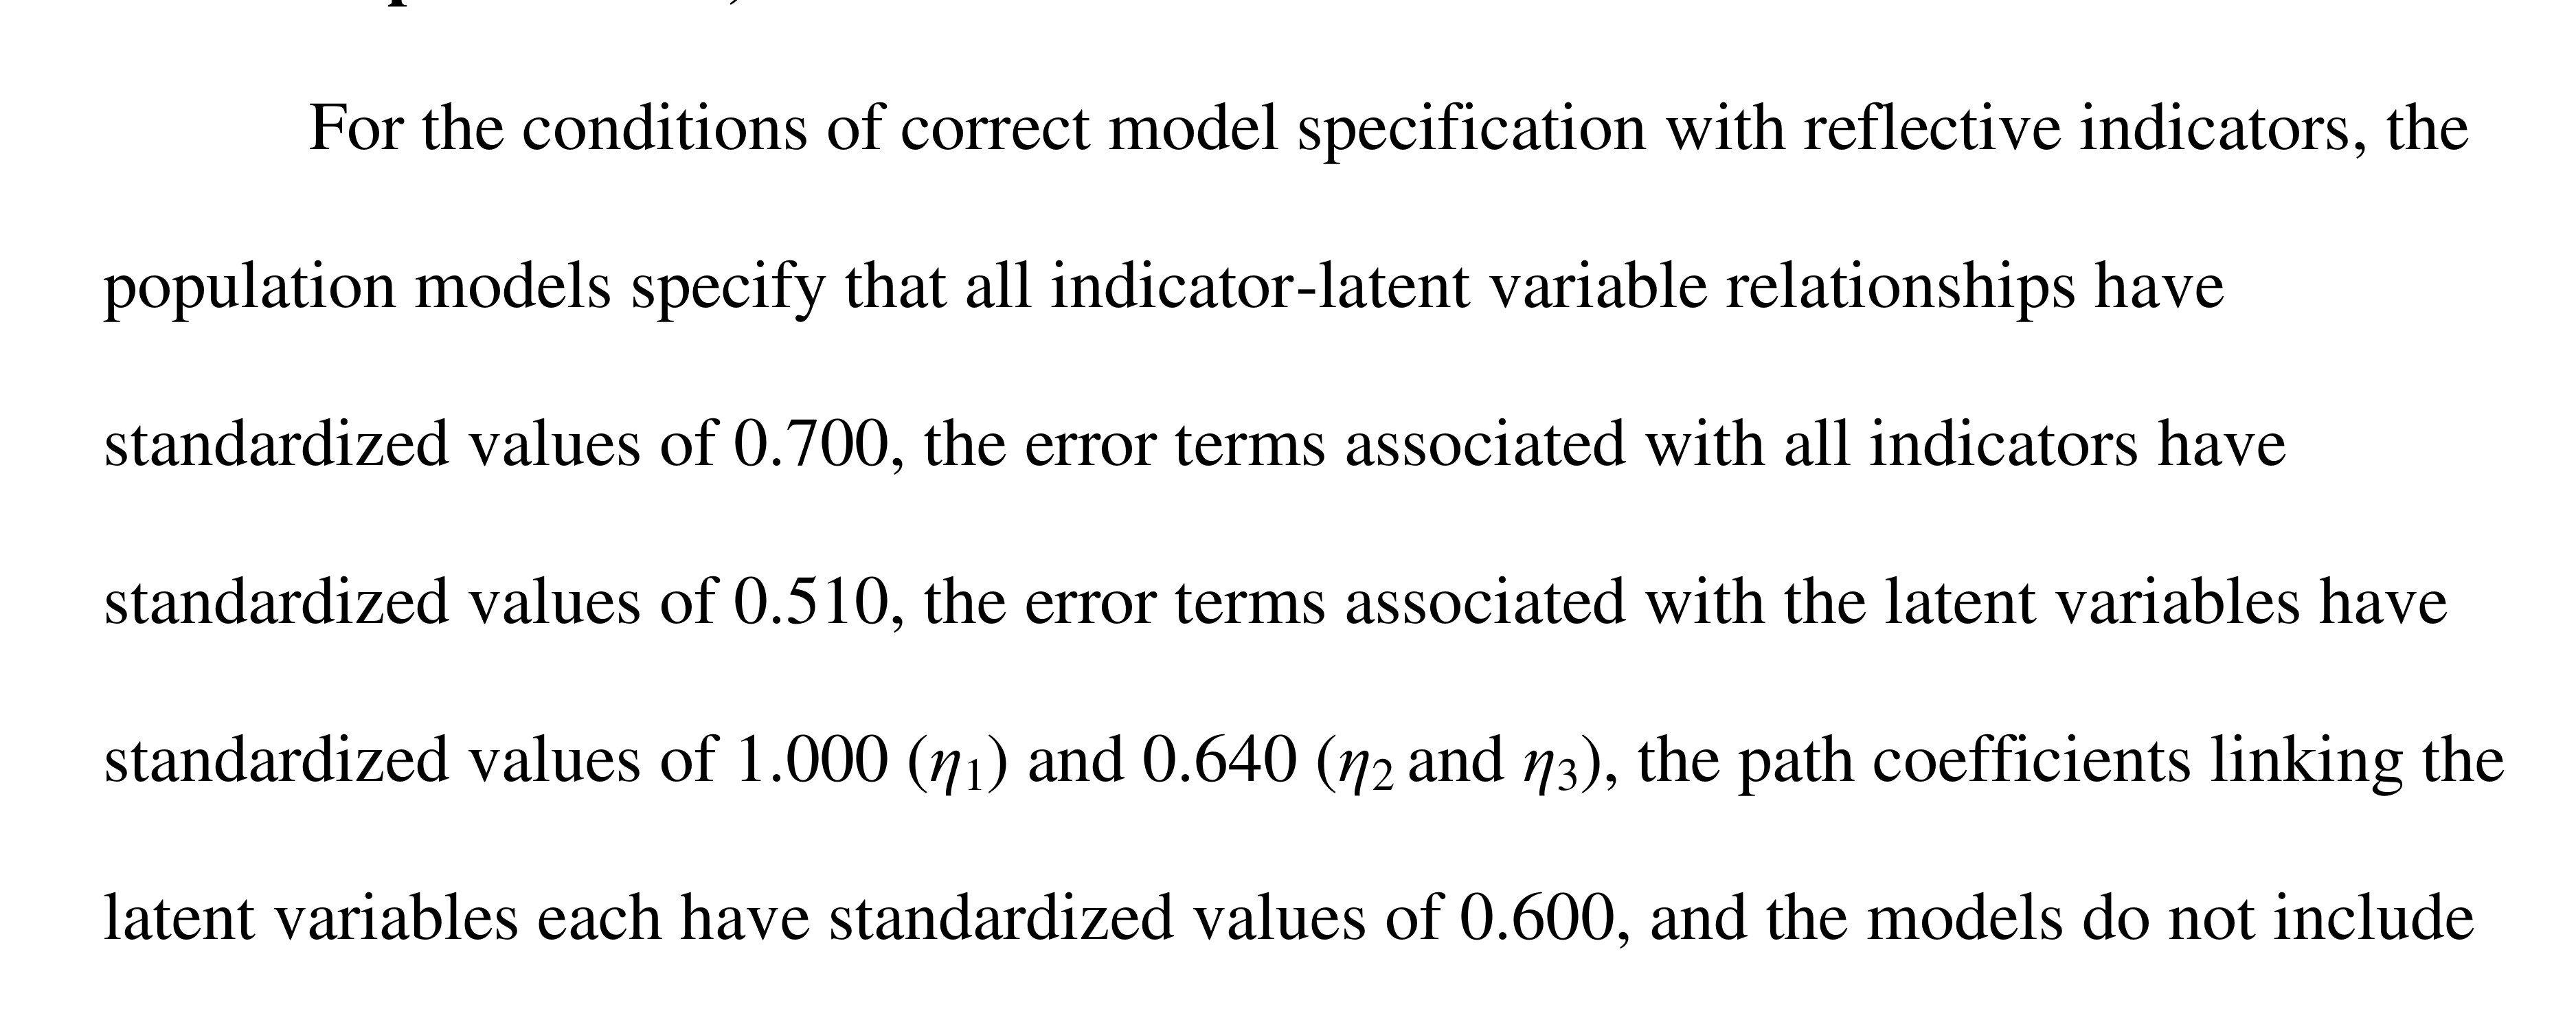
\includegraphics[width=\textwidth]{figures/population.png}
\caption{Chumney (2013), dissertation page 38. Standardized population
values for the correctly specified reflective model.}
\label{fig:population}
\end{figure}

Formative conditions are reflective indicators with unique variance 0.001.
The dissertation says so: the formative arm is an almost error-free
reflective model, so that every estimator, including partial least squares
in mode A, can be applied in the same way. Misspecification omits three
cross-loadings that are in the population. The analysis model is always
simple structure. Section~\ref{sec:cross} records which items those are and
which unstandardized cross-loading reproduces the parenthetical 0.21.

Data were drawn from the multivariate normal distribution with that
covariance, 150 times in each of the 36 conditions. The dissertation drew
the same conditions in Mplus~6. We did not have Mplus~6. Seeds are
\code{simulation/replicate.R}{40}. Replication $r$ in a cell uses
\texttt{set.seed(cell\_id + r)}.

Maximum likelihood was fit with lavaan 0.7-3, factor variances fixed at 1,
at most 1000 iterations
(\code{simulation/replicate.R}{58}).
A replication counts as converged when the optimizer converges and every
unique variance and factor residual variance is positive. Partial least
squares was fit with cSEM 0.7.1, mode A, centroid inner weights, classical
outer loadings, at most 1000 iterations
(\code{simulation/replicate.R}{94}).
Generalized structured component analysis was fit with gesca 1.0.5, at most
1000 iterations and no bootstrap
(\code{simulation/replicate.R}{131}).
A component loading outside $[-1, 1]$ was treated as an implausible
residual, which did not occur. Percent bias is
\code{simulation/replicate.R}{173}, the average of equation~(15).

The tools were chosen for the following reasons. R 4.3.3
(\url{https://cran.r-project.org/}) is the language the partial least
squares package in the dissertation runs in. lavaan 0.7-3
(\url{https://cran.r-project.org/package=lavaan}) estimates the same normal
maximum likelihood the dissertation estimated in Mplus. cSEM 0.7.1
(\url{https://cran.r-project.org/package=cSEM}) estimates partial least
squares path models. The dissertation cites the plsSEM package of Monecke
and Leisch (2012), which is semPLS on CRAN. semPLS 1.0-10 installs, and
\texttt{plsm} then errors on this R because \texttt{class()} of a matrix
has length 2 and is combined with \texttt{||}. cSEM with disattenuation
turned off returns the classical outer correlations that semPLS would have
returned. gesca 1.0.5
(\url{https://cran.r-project.org/package=gesca}) is an R implementation of
generalized structured component analysis. The dissertation used the GeSCA
program at \url{http://www.sem-gesca.org}. That host did not resolve on
29 October 2026. mvtnorm 1.4-2
(\url{https://cran.r-project.org/package=mvtnorm}) draws the normal samples.
The full grid of 36 conditions and three estimators took 929 seconds and is
stored in \filelink{simulation/out/reps150-full.rds}, commit
\texttt{06b39790bc2c658b40b6942f6c2e69bcc80a8a3b}.

The Bayesian fits use blavaan 0.6-1
(\url{https://cran.r-project.org/package=blavaan}) with rstan 2.32.7
(\url{https://cran.r-project.org/package=rstan}), because the dissertation
estimates this arm in Mplus~6 and blavaan is the R package for Bayesian
structural equation models. The iteration cap, the prior, and the
convergence rule are in Section~\ref{sec:bayes} and in
\linkbayes.

\section{What matched}
\label{sec:matched}

Do the printed percent biases reappear under the population values in
Figure~\ref{fig:population}? For maximum likelihood and partial least
squares, yes, across the item counts we checked. For generalized structured
component analysis, yes at three and five indicators per factor.

At $n=1000$, correctly specified reflective indicators, maximum likelihood
measurement percent bias is 2.730, 2.234, and 2.085 at three, five, and
seven items. The printed values are 2.712, 2.261, and 2.117. Partial least
squares is 15.919, 9.841, and 7.184, next to 15.896, 9.715, and 7.064.
The three-indicator rows are inside the Holm band in
\linkcsv. The five- and seven-item
maximum likelihood and partial least squares rows move with the printed
column by a few tenths, on a scale where the standard deviations in
Table~3 are about 0.4 to 0.8 at $n=1000$.

Partial least squares and generalized structured component analysis each
converged on all 5400 replications. The dissertation reports the same
5400/5400. Maximum likelihood converged on 4648 of 5400 replications, which
is 86.1 percent. The prose in Chapter~4 says 94 percent. The sum of
Table~1 is 5038 of 5400, which is 93.3 percent. Our shortfall relative to
Table~1 is concentrated in the formative misspecified cells with five and
seven items, and in one reflective cell discussed in
Section~\ref{sec:open}. At three items the misspecified formative counts
are 21 against 35 at $n=50$, and 102 against 119 at $n=1000$. Those two
differences have $z$ of 2.09 and 2.25. Holm within the convergence family
labels them close.

On the three-indicator slice, 20 of 24 measurement comparisons and 22 of 24
structural comparisons are matches after Holm. The two measurement rows
labeled close in the output are partial least squares and generalized
structured component analysis under misspecified reflective indicators at
$n=1000$: 19.377 and 19.371 against a printed 19.196, with $z$ about 2.4.
The absolute gaps are under 0.2 on a percent-bias scale whose interesting
contrasts are several points wide.

\section{What the goodness-of-fit bias required}
\label{sec:gof}

Which population goodness of fit is being subtracted in Table~2? For
correctly specified reflective models, the subtraction that reproduces the
printed bias uses 0.600. The subtraction that uses equations~(12)--(14) on
the standardized loadings does not.

Equation~(14) is the square root of average communality times average
$R^2$. Equation~(12) defines a block communality as the average squared
correlation of the indicators with the component. For the standardized
reflective model every correlation is 0.70, so the average communality is
0.49, the endogenous $R^2$ values are 0.36, and the goodness of fit is
$\sqrt{0.49 \times 0.36} = 0.420$. Our maximum likelihood mean at
$n=1000$ with three reflective indicators is 0.421. The printed bias is
$-0.180$. The difference $0.421 - 0.600 = -0.179$ falls inside the band
around $-0.180$. The value 0.600 is $\sqrt{1 \times 0.36}$: communality
equal to the square of the unstandardized loading 1 that the figure prints
above the parentheses, times the endogenous $R^2$ of 0.36.

The same 0.600 benchmark puts our partial least squares bias at $-0.237$
next to the printed $-0.238$. Our gesca bias in that cell is $-0.237$ next
to the printed $-0.251$. The absolute gap is 0.014. The printed standard
deviation in that gesca cell is 0.002, so the two-standard-error band is
narrow and the verdict is no match. Our standard deviation is 0.016, in
line with partial least squares in the same cell. The printed generalized
structured component analysis column is less variable than either component
method was in our run.

Misspecified cells do not fall into place under either benchmark. At
$n=1000$, three reflective indicators, omitted cross-loadings, our maximum
likelihood goodness of fit is 0.516. Minus 0.600 that is $-0.084$. Minus
the standardized population value 0.447 it is $+0.070$. The printed bias is
$+0.147$. Both readings miss, and the same sign error appears for partial
least squares and gesca. Section~\ref{sec:open} keeps that gap open.

Formative models have a standardized loading near 1, so 0.600 and the
standardized population value 0.599 agree. Printed biases in the correctly
specified formative cells are within a few thousandths of zero, and our
biases are as well.

\section{Assumptions}
\label{sec:assumptions}

Each subsection is a choice the dissertation does not pin down and that we
supplied. Turning the choice off is the check named in the subsection.

\subsection{Disturbance variance 0.3136}

The figure prints a structural disturbance of 0.31 under a standardized
value of 0.64. With factor variance 0.49, the disturbance that keeps both
factor variances equal and the standardized disturbance equal to 0.64 is
$0.49 \times 0.64 = 0.3136$. We used 0.3136. Using the printed 0.31 would
make the second factor variance 0.4864 instead of 0.49. The standardized
loading would move by less than 0.01. The match of Table~3 at $n=1000$ to
two or three decimals is the check that the rounding does not carry the
comparison.

\subsection{Nominal targets in equation (15)}

Equation~(15) divides by the population parameter. We used the standardized
values named in the text: 0.70 for every reflective loading, 1.00 for a
formative loading on a single-factor item, 0.56 for a formative loading on
a cross-loading item, and 0.60 for each path. The completely standardized
formative loading implied by unique variance 0.001 is 0.999. Comparing
estimates with 1.00 leaves a percent bias of about 0.10 that does not
shrink with $n$. Table~3 prints 0.100 for maximum likelihood in the
correctly specified formative cell at $n=1000$, with a standard deviation
printed as 0.000. Our mean is 0.102. A $z$-test was not computed, because
the printed standard deviation does not give a positive standard error.
The gap of 0.002 is the difference between 0.102 and a three-decimal
printing of a quantity that the marker model puts at 0.102.

\subsection{Centroid weights, classical outer loadings}

semPLS defaults to the centroid scheme. cSEM's centroid scheme was the one
we ran. On one sample of 1000 from the reflective model, centroid and path
weights returned the same loadings and the same paths, which is what a
chain with a single predictor for each endogenous factor leads one to
expect. Disattenuation was left off. Turning it on pulled the outer
loadings from about 0.81 back toward 0.70 and destroyed the match to the
printed partial least squares percent bias of 15.9.

\subsection{Which replications are eligible for percent bias}

Percent bias is averaged over replications that converged to positive
residual variances. The dissertation uses the same rule. Where our
convergence count is lower, the bias is the bias among the replications
lavaan accepted. At three formative misspecified indicators and $n=1000$,
that subset is 102 replications against the printed 119, and the
measurement percent bias still matches (21.686 against 21.643).

\section{Ambiguities that were resolved}
\label{sec:resolved}

\subsection{The cross-loading labeled 1 (0.21)}

Figure~\ref{fig:cross} is the arrow from $\eta_1$ to Y8 in Figure~3 of the
dissertation. The label on the arrow is 1 above and (0.21) below. The
primary loading on Y8 is 1 above and (0.70) below, and the unique variance
is 0.29. Those three parenthetical and residual values are mutually
consistent when the unstandardized cross-loading is 0.30, the factor
variance is 0.49, and the primary unstandardized loading is 1. An
unstandardized cross-loading of 1, the number printed above (0.21), does
not produce a standardized cross-loading of 0.21 together with a
standardized primary loading of 0.70.

\begin{figure}[ht]
\centering
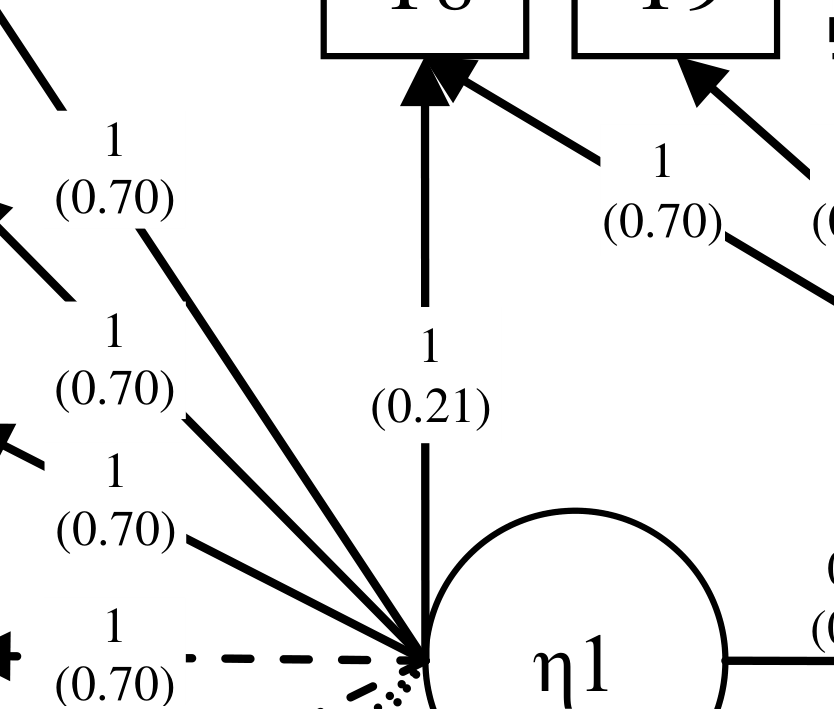
\includegraphics[width=0.72\textwidth]{figures/crossloading.png}
\caption{Chumney (2013), Figure~3, the cross-loading of Y8 on $\eta_1$.
The crop is 600 dpi, from
\linkcrop.}
\label{fig:cross}
\end{figure}

We drew the data with the unstandardized cross-loading 0.30. The
standardized values that fall out are 0.700 and 0.210, up to rounding from
a unique variance of 0.29
(\filelink{simulation/population.R},
\code{simulation/population.R}{47};
\linkcheck).
The command is \texttt{Rscript simulation/check\_standardized.R}, which
writes \texttt{simulation/out/standardized\_check.json}. The check against
the dissertation is the misspecified reflective measurement row of
Table~\ref{tab:compare}: printed 9.673, ours 9.676.
The output file is in commit \texttt{06b39790bc2c658b40b6942f6c2e69bcc80a8a3b}.

For formative misspecification the figure prints an unstandardized 1 on
both arrows of a cross-loading item, and both parenthetical standardized
values are 0.56. That pair is consistent. Our measurement percent bias in
that cell is 21.686 against the printed 21.643.

\subsection{Which indicators belong to the three-item model}

The note under Figures~1--4 says solid lines are in every condition, dashed
lines are added at five items, and dotted lines are added at seven. The
solid boxes on $\eta_2$ are Y8, Y9, and Y14: the first indicator, the second, and the last. Y8,
Y14, and Y15 are the three cross-loading items, and they are solid, so the
cross-loadings are present at every item count. The indicator sets are
\code{simulation/population.R}{6}, in commit
\texttt{06b39790bc2c658b40b6942f6c2e69bcc80a8a3b}.
The 600 dpi crop of the population
paragraph is \texttt{paper/figures/population.png}, regenerated by
\texttt{python3 paper/figures/crop\_pages.py}.

\subsection{Equation (15) is a percent}

The text layer of the PDF drops the fraction bar and the absolute-value
bars in equation~(15). The page shows
$\%\mathrm{BIAS} = \big[|\theta_i - \theta_B| / \theta_B\big] \times 100$.
Figure~\ref{fig:eq15} is the crop. Reading the formula as a proportion
rather than a percent would miss Table~3 by a factor of 100. The crop is
\texttt{paper/figures/equation15.png}.

\begin{figure}[ht]
\centering
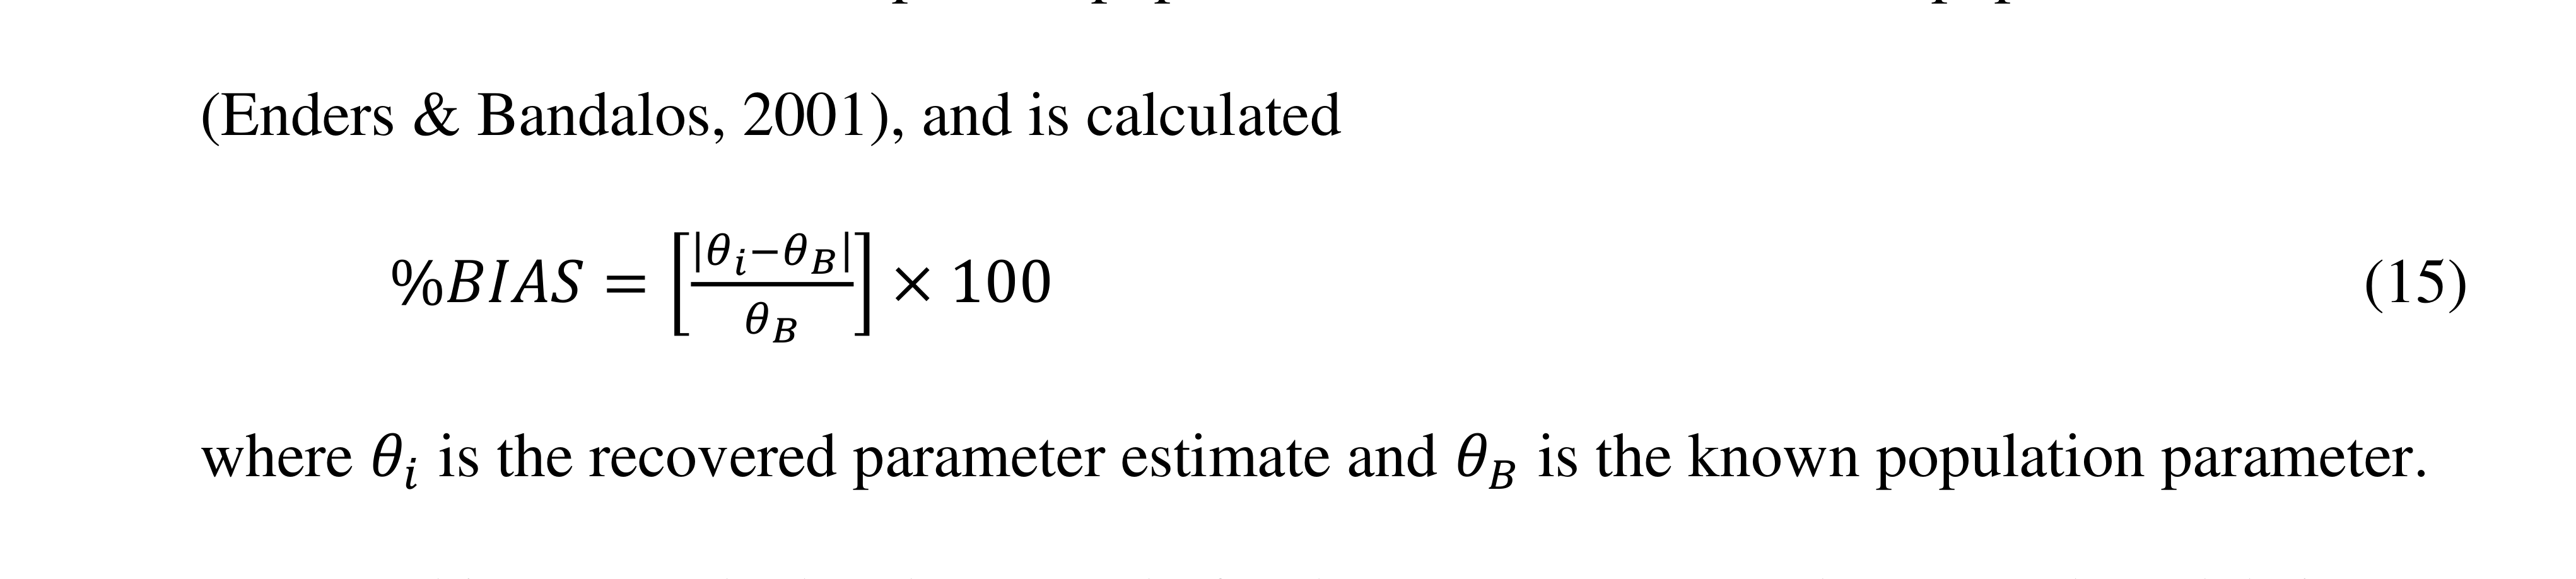
\includegraphics[width=\textwidth]{figures/equation15.png}
\caption{Chumney (2013), equation~(15), dissertation page 47 in the PDF
numbering of the body. Absolute percent bias.}
\label{fig:eq15}
\end{figure}

\section{The Bayesian subset}
\label{sec:bayes}

Do posterior means from a 1000-iteration chain recover the printed Markov
chain Monte Carlo column? The percent biases do, on the cells where the
chain mixes. The convergence counts do not, on the cells where Table~1
shows the chain failing or where the unique variances are 0.001.

The procedures section sets the maximum number of iterations to 1000 for
every estimator and estimates the Bayesian model in Mplus~6. It discusses
noninformative priors in the literature review and does not name a numeric
prior, a chain count, or a cutoff. Mplus's default priors in the Bayesian
notes the dissertation cites are a flat prior on loadings and an
inverse-gamma $(-1, 0)$ prior on variances. A Stan translation of that
variance prior, \texttt{gamma(0.01, 0.01)} on the standard deviation with
\texttt{normal(0, 1e4)} loadings, produced divergent transitions and a
potential scale reduction of 2.39 on one $n=50$ fit. The subset uses
blavaan's proper defaults instead: normal priors with mean 0 and standard
deviation 10 on loadings and regressions, and \texttt{gamma(1, 0.5)} on
residual standard deviations. Two chains, 500 burn-in iterations, and 500
retained draws make 1000 iterations. A replication counts as converged when
the largest potential scale reduction is below 1.05, Mplus's default
\texttt{BCONVERGENCE} of 0.05. The script is
\linkbayes. The run is 30 replications, the
sample sizes 50 and 1000, all four three-indicator conditions, and the
seven-indicator correct reflective cells. It took 6731 seconds. Output is
\filelink{simulation/out/bayes-reps30.rds}.

At $n=1000$ with three reflective indicators the measurement percent bias
is 2.902 (standard deviation 0.734) against the printed 2.738 (standard
deviation 0.706). The structural percent bias is 3.847 against 4.272.
Both differences are inside two standard errors. At $n=50$ with seven
reflective indicators the measurement percent bias is 10.596 against the
printed 10.202. The same cell's convergence is 30 of 30 here and 51 of 150
in Table~1. Stan's sampler reached the cutoff inside 1000 iterations on
every replication of that cell. The printed column did not.

Under formative misspecification the cutoff is missed more often here than
in Table~1: 22 of 30 at $n=50$ against 149 of 150, and 25 of 30 at
$n=1000$ against 150 of 150. The measurement percent bias among the
replications that did converge is 21.481 at $n=1000$, next to the printed
maximum likelihood value 21.643 in that cell. The dissertation pooled
maximum likelihood and Markov chain Monte Carlo for the measurement-bias
follow-ups because those two columns agreed. The subset agrees with that
pooling on the bias, and it does not agree with Table~1 on the
formative-misspecification counts.

\section{Readings of the formative structural cell}
\label{sec:formative}

Which reading of equation~(15) and of the formative model produces the
printed structural percent bias 1.196 at $n=1000$ with three items? None of
the readings below. The five-item and seven-item cells of the same printed
row, 2.623 and 2.623, are reproduced by the baseline reading.

The baseline is absolute percent bias of the two standardized paths against
0.60, factor variances fixed at 1, Heywood replications dropped. That mean
is 2.601 (standard deviation 1.447) on 150 replications, seed
\texttt{20441915}. The same seed and the same draws were refit under these
readings, in \linkform, with the
console record in \linkformout.

\begin{center}
\small
\setlength{\tabcolsep}{4pt}
\begin{tabular}{@{}p{0.62\textwidth}p{0.22\textwidth}@{}}
\toprule
Reading & Mean percent bias \\
\midrule
Factor variances fixed at 1, absolute, paths versus 0.60 & 2.601 \\
Marker identification, first loading fixed at 1, absolute & 2.601 \\
Signed percent bias, factor variances fixed at 1 & $-0.166$ \\
Signed percent bias, marker identification & $-0.166$ \\
Column-standardized data, then the baseline & 2.601 \\
Baseline, keeping replications with a nonpositive variance & 2.601 \\
Absolute bias of the mean path, rather than the mean of absolute biases & 0.166 \\
Unstandardized marker paths versus 0.60 & 3.257 \\
Paths and the two standardized residual variances & 2.761 \\
Each path alone & 2.603 and 2.599 \\
\bottomrule
\end{tabular}
\end{center}

The marker parameterization and the fixed-factor-variance parameterization
return the same standardized paths on these draws. Keeping the Heywood
replications changes nothing in this cell, because all 150 replications
had positive variances. The signed mean is $-0.166$, so the paths are
nearly unbiased and the absolute percent bias is the average size of the
sampling error. The bias of the mean path is 0.166. That summary is 0.166, and the
printed cell is 1.196.

The same baseline at five items is 2.516 against the printed 2.623, and at
seven items it is 2.628 against the printed 2.623. At $n=300$ and five
items it is 4.660 against the printed 4.658. The specification, the
absolute percent, and the treatment of improper solutions reproduce the
rest of that row. The open piece is the single printed value 1.196.

\section{Two implementations of generalized structured component analysis}
\label{sec:gsca7}

Does the printed rise at seven indicators depend on the GeSCA program?
Both R implementations we can run decline with the number of indicators,
in step with each other.

On 40 replications at $n=1000$, correct reflective model, measurement
percent bias from gesca 1.0.5 and from cSEM's GSCA option is 15.825 and
15.825 at three items, 9.838 and 9.838 at five items, and 7.040 and 7.040
at seven items
(\linkgsca,
\linkgscaout).
The 150-replication gesca means are 15.938, 9.850, and 7.189. The printed
column is 15.918, 9.734, and 13.667. Three and five items match. Seven
items is the rise that neither R implementation produces.

Turning on cSEM's disattenuation changes the seven-item mean from 7.040 to
2.106, which tracks maximum likelihood (2.085 in the 150-replication run)
rather than the printed generalized structured component analysis column.
The dissertation's component loadings are the undisattenuated ones: that
is what matches 15.9 at three items.

The host named in the dissertation, \url{http://www.sem-gesca.org}, did
not resolve on 29 October 2026. A Wayback snapshot of that host from
29 July 2023 is an HTML landing page, not a batch estimator. The successor
site \url{https://www.gscapro.com/} answered HTTP 200 and is a product
page, not a program we could run on these draws. The seven-indicator
difference is a dependence on software we cannot execute here. It is open
whether the 2013 GeSCA program would reproduce 13.667 on these draws.

\section{What remains unresolved}
\label{sec:open}

The Bayesian percent biases in Table~\ref{tab:bayes} are inside the band
where the chain mixes. The convergence proportions are not. Table~1's
Markov chain Monte Carlo count at $n=50$ with seven reflective indicators
is 51 of 150. The Stan run accepted 30 of 30. The formative
misspecification counts go the other way. A Mplus~6 input with
\texttt{BITERATIONS} set to 1000, on these seeds, would show whether the
difference is the Gibbs sampler, the improper variance prior, or the
potential scale reduction rule. The prose rate 87.7 percent and the
Table~1 sum 88.3 percent remain an internal difference in the
dissertation, as in the list below.

The goodness-of-fit bias under misspecification is open. Both benchmarks in
Section~\ref{sec:gof} miss the printed positive biases, by about 0.08 to
0.23 depending on the cell and the benchmark. The parameter estimates in
those same cells match, so the gap is in the goodness-of-fit number rather
than in the loadings. What would settle it is the program that computed the
``true'' goodness of fit, or a record of whether $\eta_1$ was given an
$R^2$ of 0 inside that average. The prose says the average runs over
$\eta_1$, $\eta_2$, and $\eta_3$. Putting a zero in for $\eta_1$ produces
$\sqrt{\bar C \times 0.24}$. For the misspecified reflective population,
$\bar C = 0.554$ and that square root is 0.365. Our estimated goodness of
fit of 0.516 minus 0.365 is 0.151, next to the printed 0.147. That reading
fits this one cell and does not fit the correctly specified reflective
cell, where the same rule would predict a bias near $+0.08$ and the table
prints $-0.180$. One formula has not covered both cells.

Maximum likelihood convergence under formative misspecification with five
and seven items is lower in our run than in Table~1, by 30 to 100
replications in a cell. At $n=50$ and seven items the table shows 134 of
150 and we accepted 34. The unique variance in the population is 0.001 and
each cross-loading item has two unstandardized loadings of 1, so lavaan's
nonpositive-variance check fires often. Mplus~6's check on the same
covariance may treat the boundary differently. The measurement percent bias
among the replications we did accept still tracks Table~3 at three items.
The original Mplus input, or the saved improper-solution flags, would
settle the count.

One reflective cell goes the other way. At $n=50$, seven items, omitted
cross-loadings, Table~1 shows 102 converged maximum likelihood replications
and we accepted 150. The $z$ against a binomial standard error is about 8.
The same population values reproduce the measurement percent bias at
$n=1000$ in that specification, so the covariance is not wildly wrong. The
open piece is again the improper-solution rule at the smallest sample.

The seven-indicator generalized structured component analysis column remains
a software difference, now checked against a second implementation.
Section~\ref{sec:gsca7} records that gesca and cSEM agree and that the
2013 GeSCA program was not runnable from this environment. The structural
percent bias in that printed cell is 4.747, and our gesca mean is 12.811,
next to our partial least squares mean of 12.747 and the printed partial
least squares mean of 12.153.

The printed structural percent bias 4.747 in that seven-indicator cell is
also the printed structural percent bias for generalized structured
component analysis at $n=300$, seven formative indicators, in the same
table. Whether one cell was typeset twice is not settled by the page. The
cell is a no match under our reading either way.

\section{A short list of internal checks}

These are comparisons inside the dissertation, kept separate from
Table~\ref{tab:compare}. They are not, by themselves, failures of the Monte
Carlo.

The prose says maximum likelihood converged for 94 percent of replications
and Markov chain Monte Carlo for 87.7 percent. Adding Table~1 gives 5038 of
5400 (93.3 percent) and 4769 of 5400 (88.3 percent). The differences are 38
and 34 replications. A misread digit in one cell would close either gap.
The 600 dpi crop of the table is \texttt{paper/figures/table1.png}.

The printed standard deviation of the formative maximum likelihood
measurement bias at $n=1000$ is 0.000. Our standard deviation is 0.003.
The means are 0.100 and 0.102.

\section{Code and source availability}

The dissertation names Mplus~6, the plsSEM package, and GeSCA at
\url{http://www.sem-gesca.org}. It does not name a repository for the
simulation script. The checks below were made on 29 October 2026.

\begin{center}
\small
\setlength{\tabcolsep}{4pt}
\begin{tabular}{@{}>{\raggedright\arraybackslash}p{0.40\textwidth}>{\raggedright\arraybackslash}p{0.16\textwidth}>{\raggedright\arraybackslash}p{0.36\textwidth}@{}}
\toprule
Place checked & UTC date & Result \\
\midrule
Dissertation PDF, procedures and references & 2026-10-29 & Obtained. The PDF contains no program file. \\
Digital Commons record cehsdiss/189 & 2026-10-29 & HTML 200. The PDF is the file. No separate code file. \\
Wayback raw file of the viewcontent PDF & 2026-10-29 & PDF obtained, 146 pages. \\
sem-gesca.org and its 2023 Wayback snapshot & 2026-10-29 & Host did not resolve. The snapshot is an HTML page. \\
gscapro.com & 2026-10-29 & HTTP 200. A product page, not a batch program. \\
GitHub user search, Frances Chumney & 2026-10-29 & No user. No repository to clone. \\
GitHub repository search for chumney & 2026-10-29 & Unrelated repositories only. \\
GitHub code search for the dissertation & 2026-10-29 & HTTP 429. The search did not finish. \\
OSF search for the title and for the author & 2026-10-29 & No records and no user. \\
Zenodo title search & 2026-10-29 & No records. \\
GitLab project search & 2026-10-29 & No projects. \\
CRAN semPLS 1.0-10 & 2026-10-29 & Source installs. \texttt{plsm} errors on R 4.3. \\
\bottomrule
\end{tabular}
\end{center}

The PDF used for the crops is
\texttt{local-extraction/literature/unl-sem/chumney2013.pdf}.
The file stays outside git. The sha256 is
\texttt{1b067efef410ac3a\allowbreak e412e3a26a7b29bf\allowbreak
1f8e50e935d21935\allowbreak 3fbe16ce8a853007}.

\section{Next steps}

The Bayesian subset leaves the convergence proportions open. A Mplus~6 run
with the iteration cap at 1000, on the seeds in
\linkbayes, would show whether Table~1's counts
are the Gibbs sampler. The seven-indicator generalized structured component
analysis column needs the 2013 GeSCA program on draws from
\filelink{simulation/population.R}. The single printed structural percent
bias 1.196 needs the Mplus output for that cell; the readings in
Section~\ref{sec:formative} did not produce it, and the neighboring cells
did match. The goodness-of-fit sign under misspecification still needs the
program that computed the population goodness of fit.

\section*{Appendix: artifacts}

\begin{center}
\small
\setlength{\tabcolsep}{4pt}
\begin{tabular}{@{}>{\raggedright\arraybackslash}p{0.32\textwidth}>{\raggedright\arraybackslash}p{0.34\textwidth}>{\raggedright\arraybackslash}p{0.26\textwidth}@{}}
\toprule
Claim & File & Command \\
\midrule
Table~\ref{tab:compare}, three-indicator bands & \path{simulation/out/comparison_i3.csv} & \path{Rscript simulation/compare.R} \\
All 36 cells, three estimators & \path{simulation/out/reps150-full.rds} & \path{Rscript simulation/replicate.R --reps 150} \\
Standardized loadings 0.70 and 0.21 & \path{simulation/out/standardized_check.json} & \path{Rscript simulation/check_standardized.R} \\
Headline, Table~1, equation~(15), cross-loading & \path{paper/figures/*.png} & \path{python3 paper/figures/crop_pages.py} \\
Bayesian subset, 30 replications & \path{simulation/out/bayes-reps30.rds} & \path{Rscript simulation/bayes_subset.R --reps 30} \\
Formative structural readings & \path{simulation/out/formative_readings.txt} & \path{Rscript simulation/investigate_formative.R} \\
gesca and cSEM GSCA at three, five, and seven items & \path{simulation/out/gsca_compare.rds} & \path{Rscript simulation/investigate_gsca.R --reps 40} \\
\bottomrule
\end{tabular}
\end{center}

\noindent
Commands are documented in \filelink{README.md}. \texttt{R\_LIBS\_USER}
must contain lavaan, cSEM, gesca, and mvtnorm. The dissertation PDF is an
argument to \texttt{crop\_pages.py} and is not in git.

\begin{thebibliography}{9}
\bibitem{chumney2013}
Frances L. Chumney.
\newblock Structural equation models with small samples: A comparative study of four approaches.
\newblock Ph.D.\ dissertation, University of Nebraska--Lincoln, 2013.
\newblock \url{https://digitalcommons.unl.edu/cehsdiss/189}.
\bibitem{monecke2012}
Armin Monecke and Friedrich Leisch.
\newblock semPLS: Structural equation modeling using partial least squares.
\newblock \emph{Journal of Statistical Software}, 48(3):1--32, 2012.
\end{thebibliography}

\end{document}
